% !TEX program = xelatex
\documentclass{article}
\usepackage{ctex}
\usepackage{listings}
\usepackage{xcolor}
\usepackage{geometry}
\usepackage{indentfirst}
\usepackage{setspace}
\usepackage{amsmath}
\usepackage{graphicx}
\usepackage{float} 
\usepackage{titlesec} 
% hyperref必须放最后
\usepackage{hyperref}
\usepackage{bookmark}

\geometry{a4paper,margin=1in}
\setlength{\parindent}{2em}
\onehalfspacing


\titleformat{\subsection}{\large}{}{0em}{}

\lstset{
    basicstyle=\ttfamily\small,
    numbers=none,
    keywordstyle=\color{black},
    commentstyle=\color{green!60!black},
    stringstyle=\color{black},
    breaklines=true,
    showstringspaces=false,
    frame=none,
    backgroundcolor=\color{gray!10},
    captionpos=b,
    columns=fullflexible,
    keepspaces=true
}

\begin{document}
% 封面
\begin{titlepage}
    \centering
    \vspace*{3cm}
    {\Huge\bfseries Week2实验报告\par}
    \vspace{10cm}
    \begin{tabular}{l l}
    班级： & \underline{\makebox[6cm]{\centering 25级计算机科学与技术}} \\[1em]
    学号： & \underline{\makebox[6cm]{\centering 25020007028}} \\[1em]
    姓名： & \underline{\makebox[6cm]{\centering 官靓颖}} \\[1em]
    任课老师： & \underline{\makebox[6cm]{\centering 周小伟}} \\[1em]
    日期： & \underline{\makebox[6cm]{\centering 2026年8月31日}}
    \end{tabular}
    \vfill
\end{titlepage}

% ========== 正文 ==========
\section*{第一部分：实验习题}
\subsection*{第一题：控制一个可清理的后台任务}
\paragraph{主题：命令行环境：进程、信号与任务控制}
\paragraph{将下方脚本保存为q05/worker.sh，再完成任务控制}
\paragraph{给定内容}
\begin{lstlisting}
#!/usr/bin/env bash
trap 'echo CLEAN_EXIT >> cleanup.log; exit 0 ' TERM INT
n=0
while true; do 
echo "$n "
n=$((n+1))
sleep 1
done
\end{lstlisting}

\subsubsection*{1.赋予脚本执行权限，在前台启动，并把stdout、stderr 分别写入stdout.log、stderr.log }
\begin{figure}[H]
    \centering
    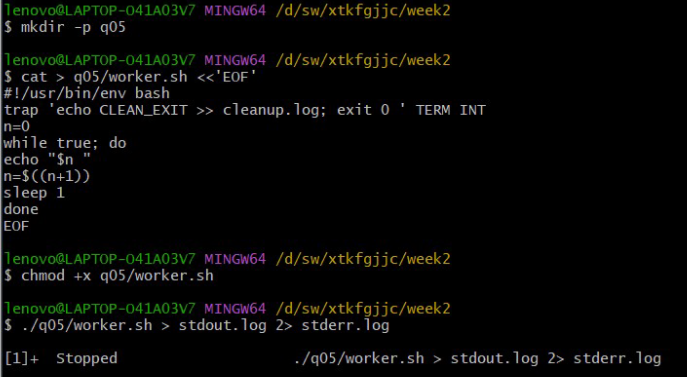
\includegraphics[width=0.7\textwidth]{0101.png}
    \caption{0101}
    \label{fig:0101}
\end{figure}
\paragraph{知识点：}
\begin{enumerate}
\item \texttt{chmod +x}：为脚本添加可执行权限
\item \texttt{>}：重定向标准输出stdout到文件
\item \texttt{2>}：重定向标准错误stderr到文件
\item \texttt{trap}捕获\texttt{SIGINT}(Ctrl‑C)、\texttt{SIGTERM}信号，收到信号执行清理逻辑写入\texttt{cleanup.log}
\end{enumerate}

\subsubsection*{2. 使用Ctrl‑Z 挂起任务，再用bg 让它在后台继续；使用jobs 确认状态}
\begin{figure}[H]
    \centering
    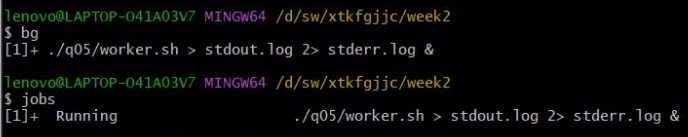
\includegraphics[width=0.7\textwidth]{0102.png}
    \caption{0102}
    \label{fig:0102}
\end{figure}
\paragraph{知识点：}
\begin{enumerate}
\item{\texttt{Ctrl+Z}发送\texttt{SIGTSTP}信号，挂起（暂停）前台作业；\texttt{bg}将挂起作业放到后台继续运行。}
\item{\texttt{jobs}查看shell会话内作业列表，显示作业编号、运行状态与命令；作业是shell层面对任务的管理。}
\end{enumerate}

\subsubsection*{3.使用jobs -p 或等价方式取得PID，不得手工抄写PID；发送SIGTERM 并等待任务结束}
\begin{figure}[H]
    \centering
    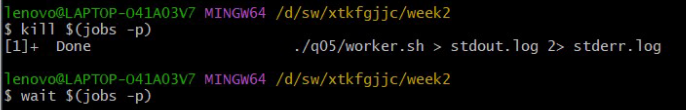
\includegraphics[width=0.7\textwidth]{0103.png}
    \caption{0103}
    \label{fig:0103}
\end{figure}
\paragraph{知识点：}
\begin{enumerate}
\item{\texttt{jobs -p}获取后台作业对应的PID；\texttt{\$(command)}命令替换，把命令输出作为参数传入。}
\item{\texttt{kill}默认发送\texttt{SIGTERM(15)}，允许程序捕获信号执行清理；\texttt{wait}等待进程结束。}
\item{\texttt{kill -9(SIGKILL)}无法被trap捕获，会直接强制销毁进程，清理逻辑不会执行，禁止使用。}
\end{enumerate}

\subsubsection*{4.确认\texttt{cleanup.log} 中出现\texttt{CLEAN\_EXIT}，且任务已经退出；禁止使用\texttt{kill -9}}
\begin{figure}[H]
    \centering
    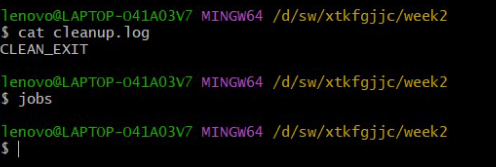
\includegraphics[width=0.7\textwidth]{0104.png}
    \caption{0104}
    \label{fig:0104}
\end{figure}
\paragraph{知识点：}
\begin{enumerate}
\item{\texttt{cat}读取文件内容，验证trap清理逻辑正常执行；\texttt{jobs}无输出代表作业已经结束。}
\item{\texttt{SIGTERM、SIGINT}可以被trap捕获实现优雅退出；\texttt{SIGKILL}信号不可捕获，无法执行清理。}
\end{enumerate}

\subsection*{第二题：语义重构与本地开发反馈}
\paragraph{主题：开发环境与工具}
\paragraph{在q06 中按照给定代码创建三个Python 文件，并使用编辑器语言服务器完成一次语义重构}
\paragraph{给定内容}
\begin{lstlisting}
# math_utils.py
def total_price(price:float , count : int) -> float : 
return price * count
# app.py
from math_utils import total_price 
print(total_price(12 .5 , 4))
# test_math_utils.py
from math_utils import total_price 
def test_total_price():
assert total_price(12 .5 , 4) == 50 .0
\end{lstlisting}

\subsubsection*{1.在已配置好Python、pytest 和ruff 的课程环境中打开q06，并启用Python 语言服务器 }
\paragraph{输入：}
\begin{lstlisting}
mkdir -p q06
cat > q06/math_utils.py <<'EOF'
def total_price(price:float , count : int) -> float : 
    return price * count
EOF
cat > q06/app.py <<'EOF'
from math_utils import total_price 
print(total_price(12.5 , 4))
EOF
cat > q06/test_math_utils.py <<'EOF'
from math_utils import total_price 
def test_total_price():
    assert total_price(12.5 , 4) == 50.0
EOF
\end{lstlisting}
\begin{figure}[H]
    \centering
    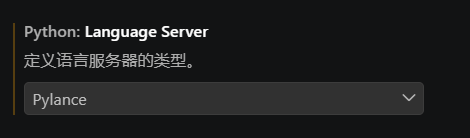
\includegraphics[width=0.8\textwidth]{02.png}
    \caption{Python语言服务器}
    \label{fig:02}
\end{figure}
\paragraph{知识点：}
\begin{enumerate}
\item{Python语言服务器(Pylance)提供静态语义分析：类型提示、代码跳转、重构能力；区别于单纯语法高亮。}
\item{\texttt{pytest}是Python单元测试框架；\texttt{ruff}是高性能linter(代码检查工具)，可检测未使用导入、格式问题。}
\end{enumerate}

\subsubsection*{2. 分别演示跳转到定义和查找引用 }
\begin{itemize}
    \item 跳转到定义：在\texttt{app.py}中光标放在\texttt{total\_price}，按下F12，跳转到\texttt{math\_utils.py}函数定义处
    \item 查找引用：光标放在\texttt{total\_price}，按下Shift+F12，列出所有引用该函数的位置
\end{itemize}
\begin{figure}[H]
    \centering
    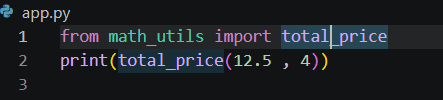
\includegraphics[width=0.8\textwidth]{03.png}
    \caption{app.py}
    \label{fig:03}
\end{figure}
\begin{figure}[H]
    \centering
    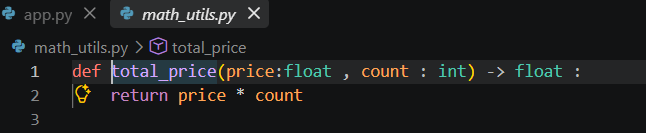
\includegraphics[width=0.8\textwidth]{04.png}
    \caption{函数定义处}
    \label{fig:04}
\end{figure}
\begin{figure}[H]
    \centering
    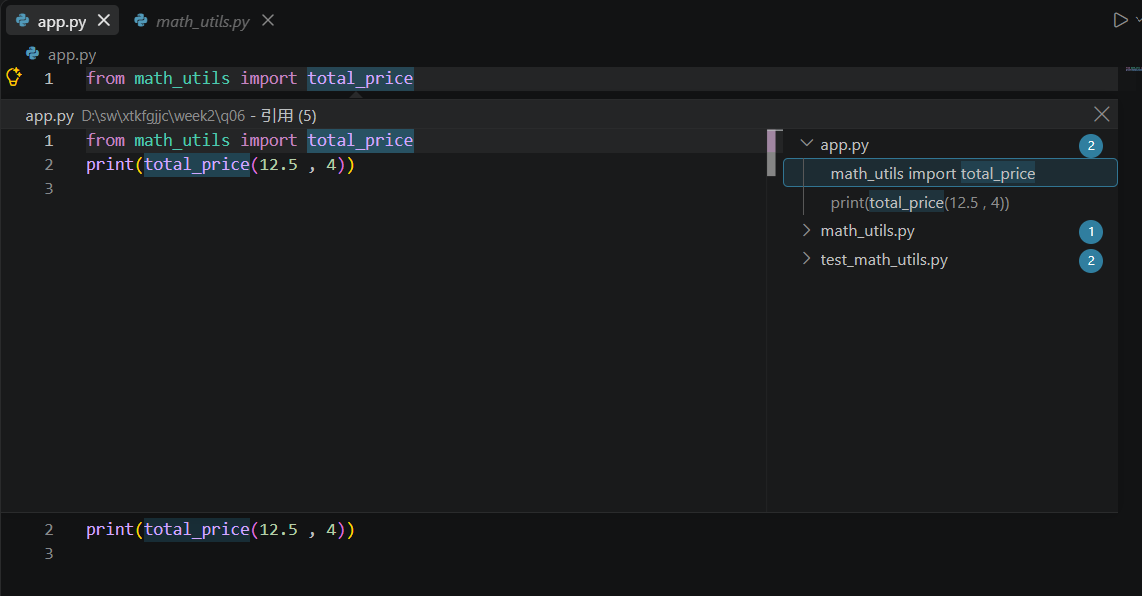
\includegraphics[width=0.8\textwidth]{05.png}
    \caption{所有引用该函数处}
    \label{fig:05}
\end{figure}
\paragraph{知识点：}
\begin{enumerate}
\item{\texttt{跳转到定义(Goto Definition)}：语言服务器找到符号的声明位置，快速定位源码。}
\item{\texttt{查找引用(Find References)}：检索项目内所有使用该符号的地方，掌握符号被哪些文件调用。}
\item{该能力由语言服务器实现，不是简单文本搜索，会识别语义，区分注释、字符串中的同名文本。}
\end{enumerate}

\subsubsection*{3.使用“重命名符号”把\texttt{total\_price} 改为\texttt{calculate\_total}，保证定义和所有代码引用同步改变 }
\paragraph{操作步骤：}
\begin{itemize}
    \item 光标放在\texttt{total\_price} 函数名上，按F2（重命名符号）
    \item 输入新名字 \texttt{calculate\_total}，回车确认
\end{itemize}
\begin{figure}[H]
    \centering
    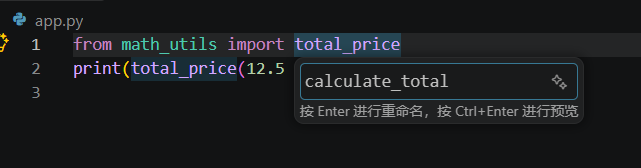
\includegraphics[width=0.8\textwidth]{06.png}
    \caption{重命名}
    \label{fig:06}
\end{figure}
\begin{figure}[H]
    \centering
    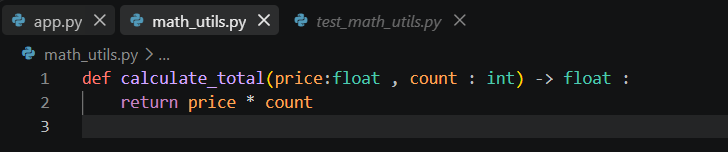
\includegraphics[width=0.8\textwidth]{07.png}
    \caption{同步改变}
    \label{fig:07}
\end{figure}
\begin{figure}[H]
    \centering
    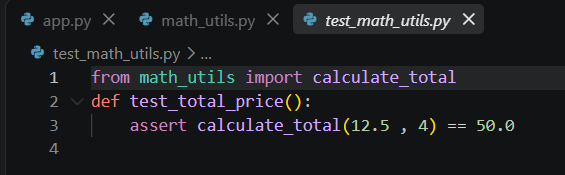
\includegraphics[width=0.8\textwidth]{08.png}
    \caption{同步改变}
    \label{fig:08}
\end{figure}
\paragraph{知识点：}
\begin{enumerate}
\item{\texttt{语义重命名(Rename Symbol)}：语言服务器提供的重构功能；会修改**所有语义上的引用**，不是单纯文本替换。}
\item{对比普通文本替换：文本替换会误改字符串、注释中同名文字；语义重命名只修改程序符号。}
\item{修改会同时更新定义、导入语句、函数调用，跨文件同步变更。}
\end{enumerate}

\subsubsection*{4.在app.py 中临时加入未使用的import os，用ruff 发现并删除；最后运行ruff 和pytest 并保证通过 }
\begin{figure}[H]
    \centering
    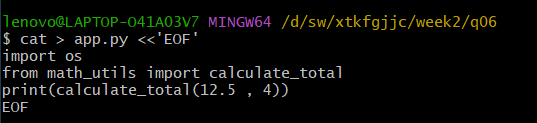
\includegraphics[width=0.8\textwidth]{020401.png}
    \caption{加入}
    \label{fig:020401}
\end{figure}
\begin{figure}[H]
    \centering
    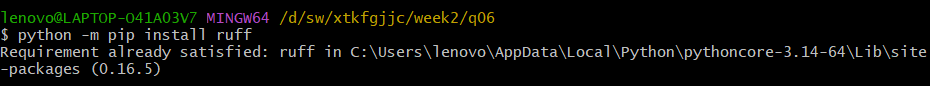
\includegraphics[width=0.8\textwidth]{020402.png}
    \caption{ruff}
    \label{fig:020402}
\end{figure}
\begin{figure}[H]
    \centering
    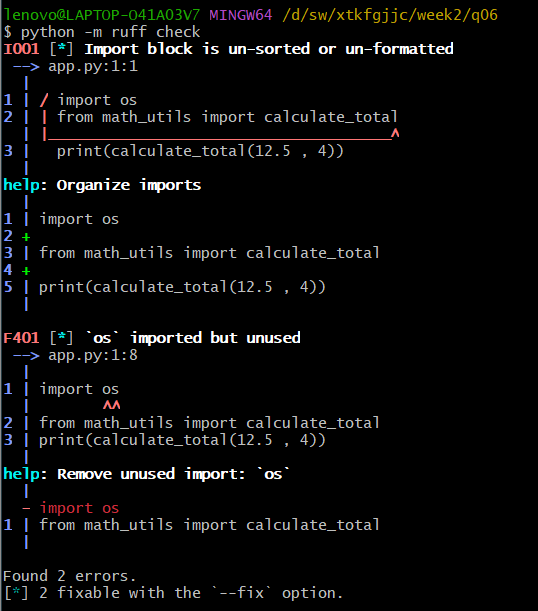
\includegraphics[width=0.8\textwidth]{020403.png}
    \caption{ruff check}
    \label{fig:020403}
\end{figure}
\begin{figure}[H]
    \centering
    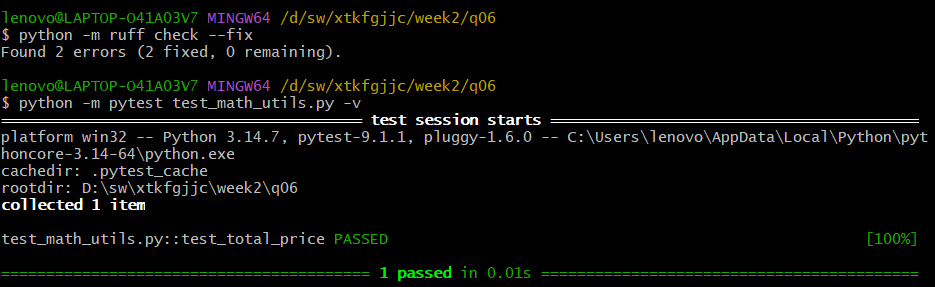
\includegraphics[width=0.8\textwidth]{020404.png}
    \caption{通过}
    \label{fig:020404}
\end{figure}
\paragraph{知识点：}
\begin{enumerate}
\item{\texttt{ruff}代码检查工具，规则F401代表：导入模块但是没有被使用。\texttt{--fix}可以自动修复部分代码问题。}
\item{\texttt{pytest}运行单元测试，断言通过代表代码逻辑没有因为重构发生错误。}
\item{静态工具(ruff)做代码质量检查；单元测试(pytest)做逻辑正确性验证，二者配合保障开发质量。}
\end{enumerate}

\subsection*{第三题：用调试器定位归并排序缺陷}
\paragraph{主题：Debugging}
\paragraph{将下列存在缺陷的归并排序代码保存为q07/merge\_sort.py，再使用调试器定位并修复}
\paragraph{给定内容}
\begin{lstlisting}
def merge(left, right):
    result = []
    i = j = 0
    while i < len(left) and j < len(right):
        if left[i] <= right[j]:
            result.append(left[i]); i += 1
        else:
            result.append(right[i]); j += 1 # 此处存在缺陷
    return result + left[i:] + right[j:]
def merge_sort(a):
    if len(a) <= 1: return a
    m = len(a) // 2
    return merge(merge_sort(a[:m]), merge_sort(a[m:]))
print(merge_sort([3, 1, 4, 1, 5, 9, 2, 6]))
\end{lstlisting}

\subsubsection*{1.先运行给定输入，确认结果错误或出现异常 }
\begin{figure}[H]
    \centering
    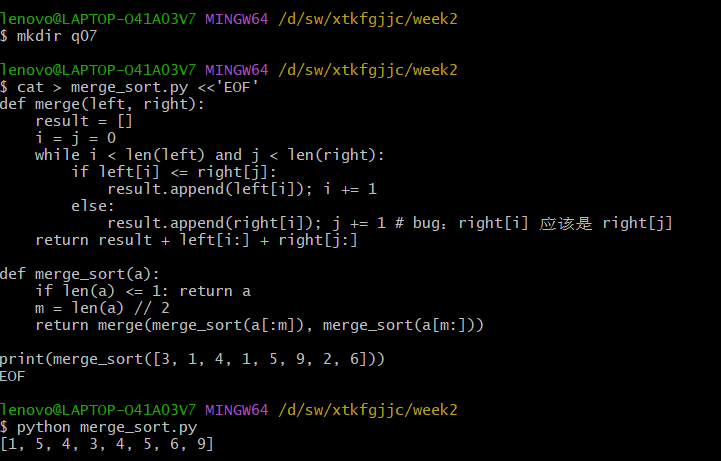
\includegraphics[width=0.8\textwidth]{0301.png}
    \caption{输出错误}
    \label{fig:0301}
\end{figure}
\paragraph{知识点：}
\begin{enumerate}
\item 错误原因：else分支中，取的是\texttt{right[i]}，应该是\texttt{right[j]}，下标变量写错，会触发列表索引越界异常。
\end{enumerate}

\subsubsection*{2.使用pdb、IDE debugger 或等价调试器，在merge 中设置断点并观察i、j、left [i]、right [j] }
\begin{figure}[H]
    \centering
    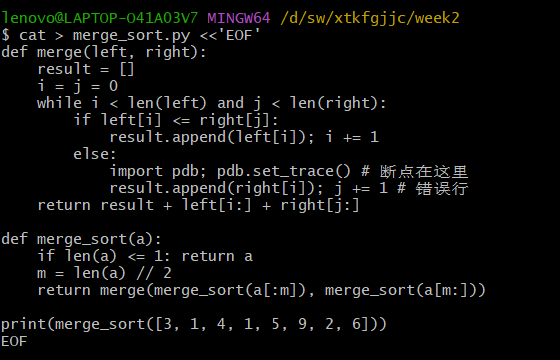
\includegraphics[width=0.8\textwidth]{0302.png}
    \caption{设置断点}
    \label{fig:0302}
\end{figure}
\begin{figure}[H]
    \centering
    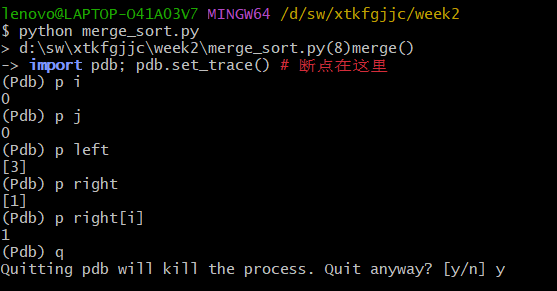
\includegraphics[width=0.8\textwidth]{0303.png}
    \caption{观察输出}
    \label{fig:0303}
\end{figure}
\paragraph{知识点：}
\begin{enumerate}
\item 调试器可以查看运行时变量的值，定位下标变量混用的逻辑错误；
\item 循环内两个数组分别使用独立指针i、j，不能混淆。
\end{enumerate}

\subsubsection*{3.完成最小修复，不得用sorted 替换归并排序 }
\begin{figure}[H]
    \centering
    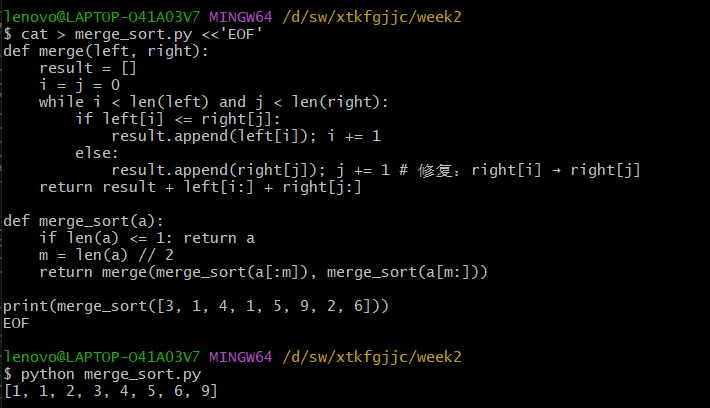
\includegraphics[width=0.8\textwidth]{0304.png}
    \caption{修复}
    \label{fig:0304}
\end{figure}
\paragraph{知识点：}
\begin{enumerate}
\item 最小修复只修改错误下标：\texttt{right[i]} 修改为 \texttt{right[j]}；
\item 归并排序核心逻辑：分治，递归拆分，合并两个有序子数组。
\end{enumerate}

\subsubsection*{4.使用pytest 增加两个测试：给定输入和含重复元素的列表；保证测试通过 }
\begin{figure}[H]
    \centering
    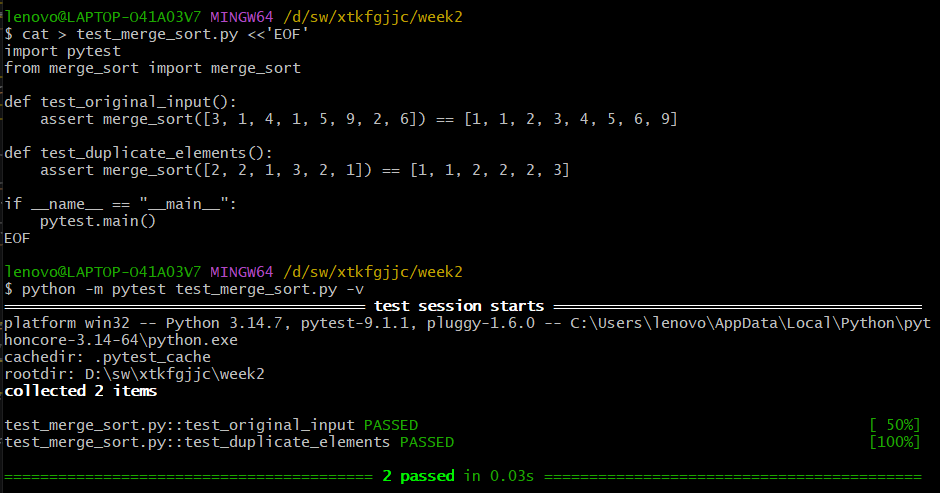
\includegraphics[width=0.8\textwidth]{0305.png}
    \caption{测试}
    \label{fig:0305}
\end{figure}
\paragraph{知识点：}
\begin{enumerate}
\item pytest用于自动化单元测试，验证排序函数正确性；
\item 测试用例需要覆盖普通序列、包含重复元素的序列，验证归并排序稳定性。
\end{enumerate}

\subsection*{第四题：先测量，再优化慢速词频程序}
\paragraph{主题：Profiling}
\paragraph{在q08 中创建可重复生成的词表和故意低效的去重程序，再使用性能分析工具优化}
\paragraph{给定内容}
\begin{lstlisting}
# generate_words.py 
import random
random.seed(20260831)
vocab = [f"w{i}" for i in range(1000)]
with open("words.txt", "w", encoding="utf-8") as f:
    f.write(" ".join(random.choice(vocab) for _ in range(30000)))
# wordfreq.py
words = open("words.txt", encoding="utf-8").read().split()
unique = []
for word in words:
    if word not in unique:
        unique.append(word)
print("count=", len(unique))
\end{lstlisting}

\subsubsection*{1.生成words.txt，使用time 运行原程序2 次并记录耗时 }
\begin{figure}[H]
    \centering
    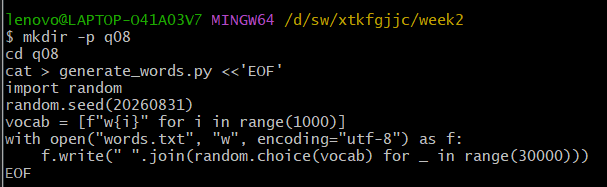
\includegraphics[width=0.8\textwidth]{0401.png}
    \caption{generate\_word.py}
    \label{fig:0401}
\end{figure}
\begin{figure}[H]
    \centering
    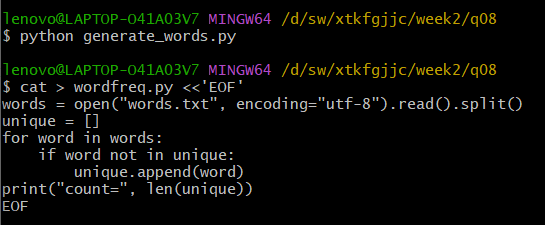
\includegraphics[width=0.8\textwidth]{0402.png}
    \caption{wordfreq.py}
    \label{fig:0402}
\end{figure}
\begin{figure}[H]
    \centering
    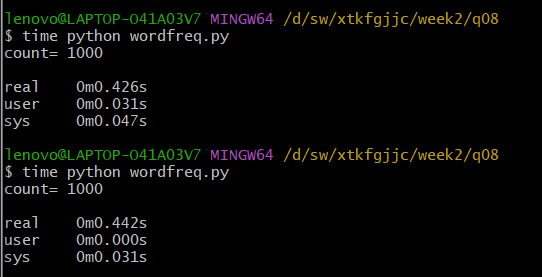
\includegraphics[width=0.8\textwidth]{0403.png}
    \caption{两次耗时}
    \label{fig:0403}
\end{figure}
\paragraph{知识点：}
\begin{enumerate}
\item 原程序使用列表\texttt{list}做去重，\texttt{word not in unique}是O(n)线性查找，遍历30000条数据时开销很大；
\item \texttt{time}工具可以测量程序实际运行耗时，多次运行减小偶然误差。
\end{enumerate}

\subsubsection*{2.使用cProfile -s cumulative 运行一次，找出主要耗时位置 }
\begin{figure}[H]
    \centering
    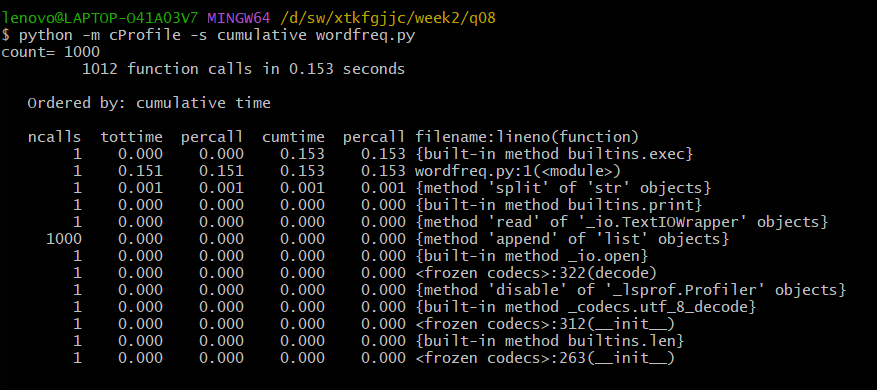
\includegraphics[width=0.8\textwidth]{0404.png}
    \caption{主要耗时位置}
    \label{fig:0404}
\end{figure}
\paragraph{知识点：}
\begin{enumerate}
\item \texttt{cProfile}是Python内置性能分析工具，\texttt{-s cumulative}按累计耗时排序；
\item 绝大部分时间消耗在循环内\texttt{word not in unique}的列表成员判断；列表查找时间复杂度O(n)。
\end{enumerate}

\subsubsection*{3.在不改变最终count 的前提下优化程序；不得写死1000 }
\begin{figure}[H]
    \centering
    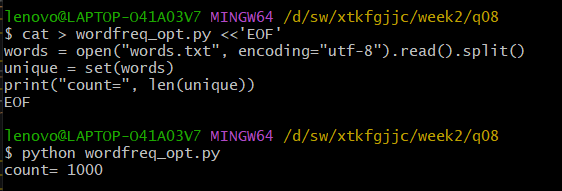
\includegraphics[width=0.8\textwidth]{0405.png}
    \caption{优化}
    \label{fig:0405}
\end{figure}
\paragraph{知识点：}
\begin{enumerate}
\item 使用Python内置\texttt{set}集合去重，集合成员查找是O(1)哈希查找；
\item 不硬编码词汇数量，仅对输入词列表做去重，输出计数结果和原程序保持一致。
\end{enumerate}

\subsubsection*{4.使用相同输入再运行2 次，计算优化前后中位数和加速比 }

\begin{figure}[H]
    \centering
    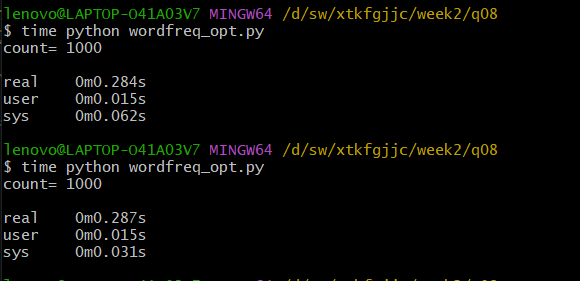
\includegraphics[width=0.8\textwidth]{0406.png}
    \caption{运行两次}
    \label{fig:0406}
\end{figure}

\paragraph{知识点：}
\begin{enumerate}
\item 原始两次real：0.426s、0.442s，中位数0.434 s，优化后两次real：0.284s、0.287s，中位数0.2855 s，加速比 $\approx$ 1.52 倍
\item Profiling性能分析流程：先测量原始耗时 $\rightarrow$ 定位性能瓶颈 $\rightarrow$ 修改算法优化 $\rightarrow$ 再次测量验证提升效果。
\end{enumerate}

% ====================== 第二部分：实验实例 ======================
\section*{第二部分 实验实例}
\subsection*{实例一：Shell参数与通配符glob}

\begin{figure}[H]
    \centering
    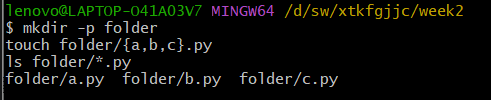
\includegraphics[width=0.8\textwidth]{001.png}
    \caption{}
    \label{fig:0406}
\end{figure}

\paragraph{知识点：}
\begin{enumerate}
\item 花括号$\{\}$通配符展开，Shell在调用程序前完成展开，传给程序的是展开后的多个参数；
\item 通配符是Shell的能力，不是命令本身的功能；
\item 区别：$*$匹配任意字符、$?$匹配单个字符。
\end{enumerate}

\subsection*{实例二：标准流重定向 stdout/stderr}

\begin{figure}[H]
    \centering
    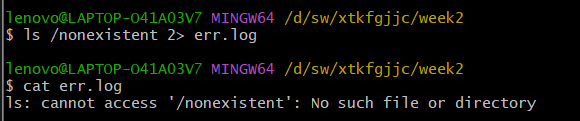
\includegraphics[width=0.8\textwidth]{002.png}
    \caption{}
    \label{fig:0406}
\end{figure}

\paragraph{知识点：}
\begin{enumerate}
\item stdout(1)正常输出，stderr(2)错误输出，二者相互独立；
\item $2>$重定向标准错误；$>$重定向标准输出；$\&>$同时重定向两者；
\item 管道$|$只会转发stdout，stderr不会进入管道。
\end{enumerate}

\subsection*{实例三：环境变量，临时环境变量 vs export导出}

\begin{figure}[H]
    \centering
    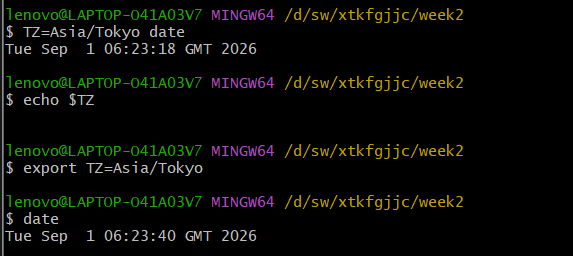
\includegraphics[width=0.8\textwidth]{00201.png}
    \caption{}
    \label{fig:0406}
\end{figure}

\begin{figure}[H]
    \centering
    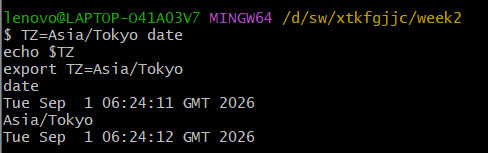
\includegraphics[width=0.8\textwidth]{00202.png}
    \caption{}
    \label{fig:0406}
\end{figure}

\paragraph{知识点：}
\begin{enumerate}
\item 命令前直接写\texttt{VAR=value cmd}：仅对该子命令生效，父Shell不会改变；
\item \texttt{export VAR=value}：把变量加入环境，所有后续子进程继承；
\item \texttt{unset VAR}删除环境变量；\texttt{printenv}查看全部环境变量。
\end{enumerate}

\subsection*{实例四：返回码 \&\& $\mid\mid$ 短路逻辑}

\begin{figure}[H]
    \centering
    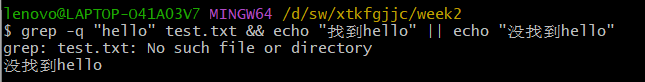
\includegraphics[width=0.8\textwidth]{004.png}
    \caption{}
    \label{fig:0406}
\end{figure}

\paragraph{知识点：}
\begin{enumerate}
\item Shell中0代表成功，非0代表失败；
\item $\&\&$：前一条返回0才执行后面；$\mid\mid$：前一条非0才执行后面；
\item \texttt{\$?}保存上一条命令的退出返回码；if语句判断也是基于返回码。
\end{enumerate}

\subsection*{实例五：信号与作业控制 Ctrl‑Z、bg、kill}

\begin{figure}[H]
    \centering
    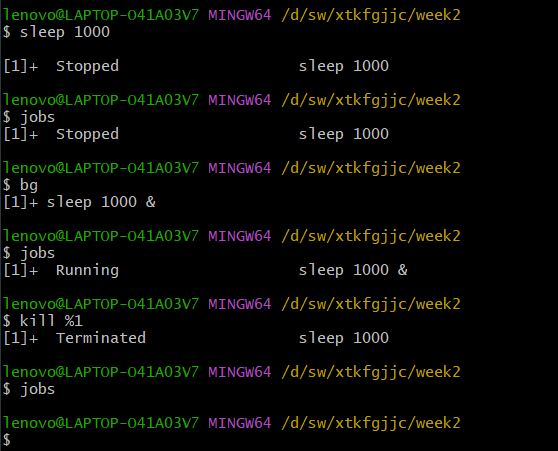
\includegraphics[width=0.8\textwidth]{005.png}
    \caption{}
    \label{fig:0406}
\end{figure}

\paragraph{知识点：}
\begin{enumerate}
\item Ctrl‑Z发送SIGTSTP，挂起进程；bg放到后台运行；fg切回前台；
\item \texttt{\%1}引用作业号；\texttt{\$!}代表最近后台作业PID；
\item SIGINT(Ctrl‑C)终止；SIGKILL不可捕获强制杀死；nohup忽略SIGHUP挂断信号。
\end{enumerate}

\subsection*{实例六：SSH远程执行命令（本地/远程区分）}

\begin{figure}[H]
    \centering
    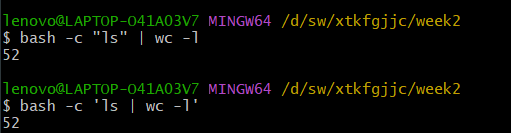
\includegraphics[width=0.8\textwidth]{006.png}
    \caption{}
    \label{fig:0406}
\end{figure}

\paragraph{知识点：}
\begin{enumerate}
\item 不加引号：管道在本地Shell解析；单引号包裹整个命令，整条命令在远程机器执行；
\item SSH密钥认证：\texttt{ssh‑keygen -t ed25519}生成密钥；\texttt{ssh‑copy‑id}推送公钥；
\item \texttt{\textasciitilde/.ssh/config}配置主机别名，scp/rsync也会读取该配置。
\end{enumerate}

\subsection*{实例七：子 shell 与命令替换 \$( )}

\begin{figure}[H]
    \centering
    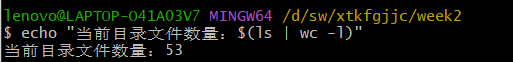
\includegraphics[width=0.8\textwidth]{007.png}
    \caption{}
    \label{fig:0406}
\end{figure}

\paragraph{知识点：}
\begin{enumerate}
\item \texttt{\$(command)} 为shell命令替换语法，先执行括号内的命令，将命令输出结果替换到字符串中。
\item 本例中先执行 \texttt{ls | wc -l} 统计当前目录文件行数，再把统计得到的数字嵌入\texttt{echo}输出。
\item 输出的数字会根据当前目录实际文件数量发生变化，示例中7仅为演示值。
\end{enumerate}

\subsection*{实例八：Shell别名alias与函数区别}

\begin{figure}[H]
    \centering
    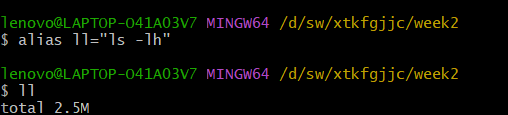
\includegraphics[width=0.8\textwidth]{008.png}
    \caption{}
    \label{fig:0406}
\end{figure}

\paragraph{知识点：}
\begin{enumerate}
\item alias只是简单文本替换，不能接收中间参数；复杂逻辑要用shell function；
\item \texttt{\textbackslash ll}可以临时绕过别名；配置写在.bashrc；\texttt{source .bashrc}重载配置；
\item dotfiles：以.开头的隐藏配置文件，存放shell/vim/tmux配置。
\end{enumerate}

\subsection*{实例九：find查找文件}

\begin{figure}[H]
    \centering
    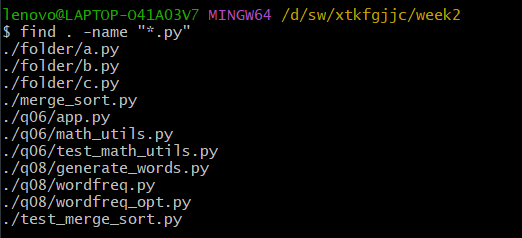
\includegraphics[width=0.8\textwidth]{009.png}
    \caption{}
    \label{fig:0406}
\end{figure}

\paragraph{知识点说明：}
\begin{enumerate}
    \item \texttt{find}：递归查找文件/目录命令。
    \item \texttt{.}：表示从当前目录开始搜索。
    \item \texttt{-name "*.py"}：匹配后缀为\texttt{.py}的文件，通配符\texttt{*}代表任意字符。
    \item 会遍历当前目录以及所有子目录，输出所有匹配的文件路径。
\end{enumerate}

\subsection*{实例十：grep文本过滤查找}

\begin{figure}[H]
    \centering
    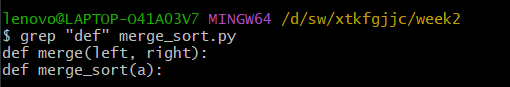
\includegraphics[width=0.8\textwidth]{0010.png}
    \caption{}
    \label{fig:0406}
\end{figure}

\paragraph{知识点说明：}
\begin{enumerate}
    \item \texttt{grep}：文本搜索工具，在文件中查找匹配指定字符串的行。
    \item \texttt{"def"}：要搜索的关键词，这里查找Python函数定义行。
    \item \texttt{merge\_sort.py}：待搜索的目标文件。
    \item 输出会打印文件中包含关键词的全部行，不匹配的行不会显示。
\end{enumerate}


\end{document}
